\documentclass[runningheads,orivec]{llncs} 
\usepackage{amsmath,amssymb,mathtools}
\usepackage{enumitem}
\usepackage{hyperref}
\usepackage{microtype}
\usepackage[T1]{fontenc}
\usepackage{booktabs}
% Figures (message-flow)
\usepackage{tikz}
\usetikzlibrary{calc,arrows.meta,positioning,calc}
\setlist[enumerate]{leftmargin=*,itemsep=0.25em}
% Algorithm boxes
\usepackage{algorithm}
\usepackage[noend]{algpseudocode}
\usepackage[section]{placeins}
\usepackage{float} % for H when absolutely needed
% dark PDF theme
\usepackage{xcolor}
\pagecolor[rgb]{0,0,0} %black
\color[rgb]{0.5,0.5,0.5} %grey

\newcommand{\prot}{\textsf{QuanTEEum}}
\newcommand{\sid}{\mathsf{sid}}
\newcommand{\Att}{\mathsf{AttestDelete}}
\newcommand{\RA}{\mathsf{RA}}
\newcommand{\FROST}{\textsf{FROST}}
\newcommand{\cFROST}{\FROST{}~\cite{komlo2020frost}}
\newcommand{\oss}{\textsf{OSS}}
\newcommand{\code}[1]{\texttt{#1}}

\begin{document}
\title{QuanTEEum: Quantum Cryptography via TEEs}
% \author{[Redacted for review]}
% \institute{[Redacted for review]}
\author{Shoaib Ahmed}
\institute{Cycles Protocol SA}
\maketitle

\begin{abstract}
One-shot signatures (OSS) have emerged as a versatile abstraction underpinning proposed blockchain applications including deterministic finality, quantum money, and ceremony-free SNARK parameters. Existing OSS constructions rely on quantum hardware that will not be widely available soon. Naïve emulations using a single trusted execution environment (TEE) inherit brittle unclonability requirements and concentrate integrity risk in one enclave. We present \prot{}, an honest-minority distributed protocol that realizes certified deletion and one-shot signing by running threshold signing entirely \emph{inside} independent TEEs. In \prot{}, $n$ enclaves run a threshold DKG, produce exactly one threshold signature on a designated statement, and each emits a remote-attestation (RA) binding an in-enclave deletion event. Security is \emph{additive}: every independent deletion attestation strictly raises the minimum attack cost, mitigating single-point TEE failures. We formalize certified deletion and one-shot signing in a remote-attestation model and show the attestation mechanism is pluggable: (a) conventional TEE RA, (b) cryptoeconomic attestations via escrowed collateral, and (c) future quantum instantiations, yielding a clean upgrade path. We sketch applications to single-shot block finality, quantum-money-flavored tokens, and de-facto ceremony-free CRS generation, and discuss liveness, freshness, and rollback subtleties.
\end{abstract}

\section{Introduction}
\paragraph{Motivation.}
OSS capture a powerful capability: make \emph{exactly-one} valid signature and then render any further signing infeasible. This single-use authenticity primitive cleanly abstracts (i) deterministic finality (each height signs once), (ii) quantum money (mint once, then unforgeable), and (iii) trusted-setup-free SNARK parameters (derive a CRS and then provably erase toxic waste). Yet today’s OSSs require quantum unclonability; TEEs offer a practical path but single-enclave designs reduce the guarantee to “trust this one box forever”.

\paragraph{Our approach.}
\prot{} lifts OSS to an \emph{honest-minority} setting by distributing the signing key across independent enclaves using a threshold DKG. The system produces one threshold signature on a frozen message and then aggregates per-enclave certified-deletion attestations bound to the session. The exact-one property reduces to the infeasibility of recovering a deleted threshold share from \emph{at least one} honest enclave, plus freshness/anti-replay for attestations.

\paragraph{Contributions.}
\begin{itemize}[leftmargin=*,itemsep=0.25em,topsep=0.25em]
  \item A formalization of certified deletion and one-shot signing in a remote-attestation model with explicit freshness and context binding.
  \item \prot{}: a threshold-in-TEE protocol that yields \emph{exactly one} threshold signature and a set of deletion attestations; security is additive across heterogeneous TEEs.
  \item A pluggable attestation mechanism: TEE RA today; cryptoeconomic attestations; future quantum erasure attestations---preserving the OSS API.
  \item Application sketches for (i) deterministic finality, (ii) quantum-money-style tokens, and (iii) de-facto ceremony-free CRS derivations.
  \item A discussion of liveness under abort, anti-replay, rollback resistance, and heterogeneity as defense-in-depth.
\end{itemize}

\section{Background and Model}
\subsection{One-shot signatures in brief}
An \oss{} scheme exposes $(\mathsf{Setup},\mathsf{KeyGen},\mathsf{SignOnce},\mathsf{Verify})$ with the property that for any keypair, at most one signature on at most one message is computationally feasible. Security is captured by a game where the adversary, after arbitrary queries \emph{except} a second signing, fails to produce two distinct valid signatures or one valid signature after certified deletion.

\subsection{Threshold signatures \cFROST{}}
We assume a Schnorr-style $t$-of-$n$ threshold signature with a secure DKG (e.g., \FROST{}). Parties hold additive shares $\{sk_i\}$ with public key $pk$, and interactive signing produces $\sigma$ on message $m$. Unforgeability holds if fewer than $t$ shares leak and nonces are not reused.

\subsection{TEE trust and remote attestation}
Each party $P_i$ hosts an enclave $E_i$ implementing \prot{}. We assume:
\begin{itemize}[leftmargin=*,itemsep=0.25em]
  \item \textbf{Code identity}: attestation binds a code measurement and the \emph{auxiliary reportdata} to outputs; verifier policy is committed via $\mathsf{policy\_hash}$ in $\mathsf{sid}$.
  \item \textbf{Sealed state semantics}: used only pre-signing to persist the DKG result across a crash.
  \item \textbf{Freshness/anti-replay}: a monotonic epoch is available (hardware counter or external append-only anchor) and is bound into attestations as a counter $\mathsf{ctr}\in\{0,1,2\}$ corresponding to JOIN, DKG, and DEL.
  \item \textbf{Deletion API}: an enclave can make shares unrecoverable (\emph{zeroization}) and prove the transition with an attestation carrying auxiliary data.
\end{itemize}
We \emph{do not} assume perfect side-channel resistance or that all rollback vectors are impossible; instead we bind acceptance to the \emph{freshness predicate} and to a one-shot latch.

\paragraph{Assumption (Replay protection \textsf{Fresh}).}
There exists a predicate $\textsf{Fresh}(\mathsf{RA},\mathsf{sid})\!\in\!\{0,1\}$ enforcing per-$(\mathsf{sid},\mathsf{eid})$ \emph{uniqueness} and \emph{strict counter monotonicity} $0\!\rightarrow\!1\!\rightarrow\!2$. The verifier accepts at most one quote for each $(\mathsf{sid},\mathsf{eid},\mathsf{ctr})$ and any $\mathsf{ctr}{=}2$ (DEL) must be fresh relative to previously accepted $\mathsf{ctr}\in\{0,1\}$. No trusted time is required; realizations include enclave-backed monotonic storage or an external append-only anchor.

\subsection{Adversary and network}
The network is asynchronous with eventual delivery. The adversary may statically corrupt up to $f$ enclaves and their hosts and is rushing. We target $t=n$ for strongest one-shot semantics; extensions to $t<n$ are discussed in \S\ref{sec:discussion}.

\section{\prot{} Protocol}\label{sec:protocol}

\begin{figure}[!htbp]
\centering
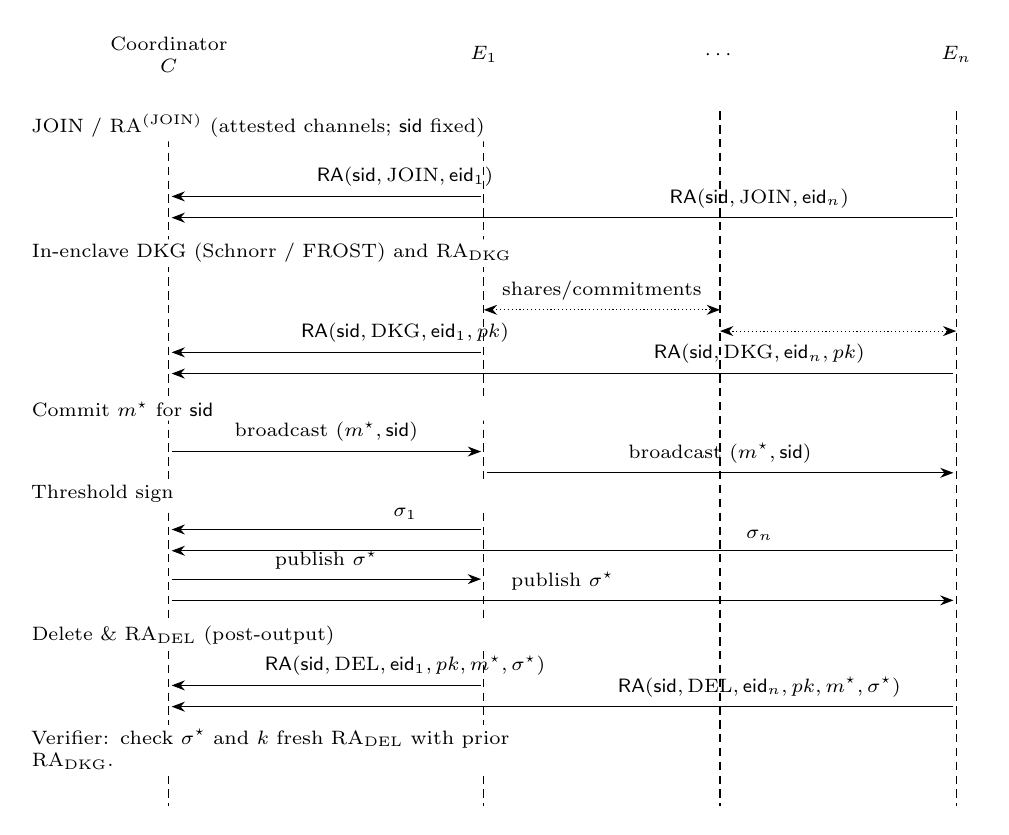
\begin{tikzpicture}[
  x=2.0cm,y=0.9cm,>=Stealth,
  every node/.style={font=\scriptsize},
  msg/.style={->,line width=0.4pt,shorten >=1pt,shorten <=1pt},
  lifeline/.style={densely dashed,line width=0.4pt},
  ann/.style={anchor=west,fill=white,inner sep=1.5pt,rounded corners=1pt,text width=6.2cm}
]
  % Column labels (kept separate from lifeline anchors)
  \node[align=center] (C_lbl)  at (0,0)   {Coordinator\\$C$};
  \node[align=center] (E1_lbl) at (2,0)   {$E_1$};
  \node[align=center] (Ed_lbl) at (3.5,0) {$\cdots$};
  \node[align=center] (En_lbl) at (5,0)   {$E_n$};

  % Lifeline anchors start below labels to avoid overlap
  \coordinate (C)  at (0,-0.8);
  \coordinate (E1) at (2,-0.8);
  \coordinate (Ed) at (3.5,-0.8);
  \coordinate (En) at (5,-0.8);

  % Lifelines
  \draw[lifeline] (C)  -- +(0,-9.8);
  \draw[lifeline] (E1) -- +(0,-9.8);
  \draw[lifeline] (Ed) -- +(0,-9.8);
  \draw[lifeline] (En) -- +(0,-9.8);

  % LEFT-MARGIN ANNOTATIONS (white boxes) to avoid any overlap with arrows
  \node[ann] at (-0.9,-1.0) {JOIN / RA$^{(\mathrm{JOIN})}$ (attested channels; $\mathsf{sid}$ fixed)};
  \node[ann] at (-0.9,-2.8) {In-enclave DKG (Schnorr / FROST) and RA$_\mathrm{DKG}$};
  \node[ann] at (-0.9,-5.0) {Commit $m^{\star}$ for $\mathsf{sid}$};
  \node[ann] at (-0.9,-6.2) {Threshold sign};
  \node[ann] at (-0.9,-8.2) {Delete \& RA$_\mathrm{DEL}$ (post-output)};
  \node[ann] at (-0.9,-9.8) {Verifier: check $\sigma^{\star}$ and $k$ fresh RA$_\mathrm{DEL}$ with prior RA$_\mathrm{DKG}$.};

  % 1) JOIN / RA_0
  \draw[msg] ($(E1)+(0,-1.2)$) -- node[above,sloped,near start]{$\RA(\mathsf{sid},\mathrm{JOIN},\mathsf{eid}_1)$} ($(C)+(0,-1.2)$);
  \draw[msg] ($(En)+(0,-1.5)$) -- node[above,sloped,near start]{$\RA(\mathsf{sid},\mathrm{JOIN},\mathsf{eid}_n)$} ($(C)+(0,-1.5)$);

  % 2) DKG (peer-to-peer) + RA_DKG
  \draw[<->,densely dotted,line width=0.4pt] ($(E1)+(0,-2.8)$) -- node[above]{shares/commitments} ($(Ed)+(0,-2.8)$);
  \draw[<->,densely dotted,line width=0.4pt] ($(Ed)+(0,-3.1)$) -- ($(En)+(0,-3.1)$);
  \draw[msg] ($(E1)+(0,-3.4)$) -- node[above,sloped,near start]{$\RA(\mathsf{sid},\mathrm{DKG},\mathsf{eid}_1,pk)$} ($(C)+(0,-3.4)$);
  \draw[msg] ($(En)+(0,-3.7)$) -- node[above,sloped,near start]{$\RA(\mathsf{sid},\mathrm{DKG},\mathsf{eid}_n,pk)$} ($(C)+(0,-3.7)$);

  % 3) Commit (freeze message for this sid)
  \draw[msg] ($(C)+(0,-4.8)$) -- node[above,sloped]{broadcast $(m^{\star},\mathsf{sid})$} ($(E1)+(0,-4.8)$);
  \draw[msg] ($(E1)+(0,-5.1)$) -- node[above,sloped]{broadcast $(m^{\star},\mathsf{sid})$} ($(En)+(0,-5.1)$);

  % 4) Sign (partials to aggregate)
  \draw[msg] ($(E1)+(0,-5.9)$) -- node[above,sloped,near start]{$\sigma_1$} ($(C)+(0,-5.9)$);
  \draw[msg] ($(En)+(0,-6.2)$) -- node[above,sloped,near start]{$\sigma_n$} ($(C)+(0,-6.2)$);
  \draw[msg] ($(C)+(0,-6.6)$) -- node[above,sloped]{publish $\sigma^{\star}$} ($(E1)+(0,-6.6)$);
  \draw[msg] ($(C)+(0,-6.9)$) -- node[above,sloped]{publish $\sigma^{\star}$} ($(En)+(0,-6.9)$);

  % 5) Certified deletion & RA_DEL
  \draw[msg] ($(E1)+(0,-8.1)$) -- node[above,sloped,near start]{$\RA(\mathsf{sid},\mathrm{DEL},\mathsf{eid}_1,pk,m^{\star},\sigma^{\star})$} ($(C)+(0,-8.1)$);
  \draw[msg] ($(En)+(0,-8.4)$) -- node[above,sloped,near start]{$\RA(\mathsf{sid},\mathrm{DEL},\mathsf{eid}_n,pk,m^{\star},\sigma^{\star})$} ($(C)+(0,-8.4)$);
\end{tikzpicture}
\caption{QuanTEEum message flow: RA$^{(\mathrm{JOIN})}$ (JOIN), RA$_\mathrm{DKG}$ (bind $pk$), Commit $m^{\star}$, Sign, RA$_\mathrm{DEL}$ (delete).}
\label{fig:flow}
\end{figure}

\paragraph{Roles.}
Parties $\{P_1,\dots,P_n\}$ run enclaves $\{E_1,\dots,E_n\}$.
A (rotating) coordinator $C$ orchestrates rounds but learns no secrets.
All protocol traffic (JOIN, DKG, Commit, Sign, Delete) is carried over
\emph{attested secure channels} (e.g., RA–TLS) whose channel binding includes an
ephemeral enclave public key $\mathsf{eid}$ attested by the enclave.

\paragraph{Session binding.}
We use DKG-first. A session identifier $\mathsf{sid}$ is derived
\[
  \mathsf{sid} \gets H(\mathsf{suite}\,\|\,\mathsf{policy\_hash}\,\|\,\mathsf{nonce}),
\]
and is embedded in all protocol messages and in the attestation \emph{reportdata}.
Here $\mathsf{nonce}$ is a fresh 128-bit value chosen by $C$ at JOIN.
The designated message $m^{\star}$ is \emph{frozen later} by a Commit step
(after DKG and before signing) and appears in the deletion attestation.

\paragraph{Parameters.}
\begin{itemize}[leftmargin=*,itemsep=0.25em]
  \item $\mathsf{suite}$: cryptographic suite identifier (curve/group, hash, domain separators, transcript encoding, threshold-signing variant).
  \item $\mathsf{policy}$: canonical verifier policy (e.g., $n,t$, minimum $\mathsf{DEL}$ attestations $k$, vendor/diversity constraints, RA roots, allowed measurements, freshness-oracle details).
  \item $\mathsf{policy\_hash} := H(\mathsf{policy})$ (committed by $\mathsf{sid}$).
  \item $\mathsf{nonce}$: 128-bit coordinator nonce ensuring $\mathsf{sid}$ uniqueness.
  \item $\mathsf{eid}$: enclave’s attested ephemeral DH/public key (per session), also used to bind the RA–TLS channel.
\end{itemize}

\paragraph{Attestation reportdata (aux).}
We use \emph{phases} $\mathsf{phase}\in\{\mathsf{JOIN},\mathsf{DKG},\mathsf{DEL}\}$ in the reportdata; no counters/timestamps.
All encodings are length-delimited and unambiguous.
\begin{align*}
  \text{RA}^{(\mathrm{JOIN})}\!:\ & \mathsf{aux} = (\mathsf{sid},\ \mathsf{phase}=\mathsf{JOIN},\ \mathsf{eid}) \\
  \text{RA}^{(\mathsf{DKG})}\!:\ & \mathsf{aux} = (\mathsf{sid},\ \mathsf{phase}=\mathsf{DKG},\ \mathsf{eid},\ pk) \\
  \text{RA}^{(\mathrm{DEL})}\!:\ & \mathsf{aux} = (\mathsf{sid},\ \mathsf{phase}=\mathsf{DEL},\ \mathsf{eid},\ pk,\ m^{\star},\ \sigma^{\star})
\end{align*}
Intuition: RA$^{(\mathrm{JOIN})}$ gates participation and binds $\mathsf{eid}$ to $\mathsf{sid}$; RA$^{(\mathsf{dkg})}$ binds the DKG result $pk$ to $\mathsf{sid}$ and $\mathsf{eid}$;
RA$^{(\mathrm{DEL})}$ certifies deletion \emph{after} producing the unique output $(m^{\star},\sigma^{\star})$.

\paragraph{Freshness and anti-replay.}
We rely on an append-only \emph{freshness oracle} (e.g., transparency log or notary quorum) that stores
entries keyed by $(\mathsf{sid},\mathsf{phase},\mathsf{eid}) \mapsto \text{digest(quote)}$ and enforces:
(i) \emph{uniqueness}: at most one entry per key; and
(ii) \emph{order}: for each $(\mathsf{sid},\mathsf{eid})$, $\mathsf{DKG}$ must precede $\mathsf{DEL}$ (JOIN optional).
Verifiers reject any $\mathsf{DEL}$ without a prior $\mathsf{DKG}$ for the same $(\mathsf{sid},\mathsf{eid})$.

\paragraph{Policy checks:}
\begin{description}
  \item[\textbf{JOIN:}] $C$ broadcasts $(\mathsf{suite},\mathsf{policy},\mathsf{nonce},\mathsf{sid})$.
  Each enclave locally admits $\mathsf{policy}$ (e.g., allowlist or operator-signed), then emits RA$^{(\mathrm{JOIN})}$.
  $C$ proceeds only with enclaves whose RA$^{(\mathrm{JOIN})}$ verifies and whose $\mathsf{sid}$ matches.
  \item[\textbf{DKG:}] Enclaves run DKG over RA-bound channels; after DKG each emits RA$^{(\mathsf{dkg})}$ with $(\mathsf{sid},\mathsf{DKG},\mathsf{eid},pk)$.
  $C$ ensures all RA$^{(\mathsf{dkg})}$ bind to the same $(\mathsf{sid},pk)$.
  \item[\textbf{Verification:}] An external verifier recomputes $\mathsf{policy\_hash}$ from its configured $\mathsf{policy}$,
  checks that $\mathsf{sid}$ commits to it, and accepts iff:
  \begin{enumerate}
    \item[(a)] $\mathsf{Verify}(pk,m^{\star},\sigma^{\star})=1$,
    \item[(b)] there are at least $k$ valid RA$^{(\mathrm{DEL})}$ with distinct $\mathsf{eid}$ satisfying diversity constraints, and
    \item[(c)] each such $\mathsf{eid}$ has a prior RA$^{(\mathsf{DKG})}$ in the freshness oracle for the same $(\mathsf{sid},pk)$.
  \end{enumerate}
\end{description}

\subsection*{Interfaces and notation}
\begin{itemize}[leftmargin=*,itemsep=0.25em]
  \item $\textsf{RA.GenQuote}(\mathsf{aux}) \rightarrow \mathsf{RA}$:
  produce a vendor-signed attestation over the enclave measurement and the byte string $\mathsf{aux}$.

  \item $\textsf{RA.Verify}(\mathsf{RA};\ \textsf{allow\_meas},\ \textsf{roots}) \in \{0,1\}$:
  verify signature under trusted RA roots and check the code measurement against the allowlist.

  \item $\textsf{Oracle.Append}(\mathsf{sid},\mathsf{phase},\mathsf{eid},\mathsf{RA})
  \in \{\mathsf{ok},\mathsf{dup},\mathsf{order\_err}\}$:
  append the quote’s digest to the append-only freshness oracle keyed by $(\mathsf{sid},\mathsf{phase},\mathsf{eid})$;
  returns $\mathsf{dup}$ on a repeat key and $\mathsf{order\_err}$ if $\mathsf{DEL}$ lacks a prior $\mathsf{DKG}$.

  \item $\textsf{Latch}(\sid,m^{\star})$:
  bind $m^{\star}$ for this session inside the enclave; subsequent signing attempts under the same $\sid$ abort.

  \item $\textsf{Del}()$:
  irrecoverably zeroize the in-enclave key material and nonces (invoked before RA$^{(\mathrm{DEL})}$).
\end{itemize}

\subsection{Setup and DKG}
\begin{enumerate}[leftmargin=*,itemsep=0.25em]
  \item \textbf{Roster selection (policy-based).} The coordinator $C$ selects a set of enclaves $\{E_i\}$ that satisfy $\mathsf{policy}$ (diversity, allowlisted measurements, RA roots).
  \item \textbf{JOIN.} Each invited $E_i$ establishes an RA–bound secure channel (RA–TLS) with ephemeral $\mathsf{eid}_i$ and emits
        RA$^{(\mathrm{JOIN})}$ with $\mathsf{aux}=(\mathsf{sid},\mathsf{JOIN},\mathsf{eid}_i)$.
  \item \textbf{Peer vetting of JOIN.} $C$ distributes the set of RA$^{(\mathrm{JOIN})}$ quotes to all $E_i$.
        Each $E_i$ verifies that all quotes validate under trusted roots, share the same $\mathsf{sid}$,
        and that the \emph{set} of participants satisfies $\mathsf{policy}$. Enclaves abort if checks fail.
  \item \textbf{DKG.} The enclaves run a Schnorr-threshold DKG (e.g., \FROST{}) entirely in\mbox{-}enclave over the attested channels,
        obtaining additive shares $\{sk_i\}$ and group public key $pk$. Shares remain only in enclave memory; optionally seal $sk_i$ until Commit/Sign.
  \item \textbf{Bind DKG result.} Each $E_i$ emits RA$^{(\mathsf{DKG})}$ with $\mathsf{aux}=(\mathsf{sid},\mathsf{DKG},\mathsf{eid}_i,pk)$;
        $C$ proceeds only if all quotes verify and bind to the same $(\mathsf{sid},pk)$, and appends them to the freshness oracle.
\end{enumerate}

\begin{algorithm}[!htbp]
\caption{\prot{}: \emph{SetupAndDKG} (inside enclave $E_i$)}
\label{alg:setup}
\begin{small}
\begin{algorithmic}[1]
\State Receive roster invitation and $(\mathsf{suite},\mathsf{policy},\mathsf{nonce},\mathsf{sid})$ from $C$.
\State Measure code $\mathsf{meas}$; generate ephemeral $\mathsf{eid}_i$; establish RA--TLS channel bound to $\mathsf{eid}_i$.
\State $\mathsf{RA}^{(\mathrm{JOIN})}_i \gets \textsf{RA.GenQuote}\big((\mathsf{sid},\mathsf{JOIN},\mathsf{eid}_i)\big)$; send to $C$.
\State Receive the set $\{\mathsf{RA}^{(\mathrm{JOIN})}_j\}_j$ for all invited enclaves from $C$; for each, run \textsf{RA.Verify} and check same $\mathsf{sid}$ and that the set satisfies $\mathsf{policy}$; abort on failure.
\State Run in\mbox{-}enclave Schnorr-threshold DKG (e.g., \FROST{}) $\rightarrow$ local share $sk_i$ and group $pk$.
\State Optionally \emph{seal} $sk_i$ until Commit/Sign; never export $sk_i$.
\State $\mathsf{RA}^{(\mathsf{DKG})}_i \gets \textsf{RA.GenQuote}\big((\mathsf{sid},\mathsf{DKG},\mathsf{eid}_i,pk)\big)$; send to $C$.
\State $\textsf{Oracle.Append}(\mathsf{sid},\mathsf{DKG},\mathsf{eid}_i,\mathsf{RA}^{(\mathsf{DKG})}_i)$.
\State \textbf{return} $pk$ (to the application/coordinator); \textbf{never} reveal $sk_i$.
\end{algorithmic}
\end{small}
\end{algorithm}

\subsection{Single-signing phase}
\begin{enumerate}[leftmargin=*,itemsep=0.25em]
  \item \textbf{Commit.} $C$ (over the RA–bound channel) broadcasts $(m^{\star},\mathsf{sid})$ for the \emph{existing} session $\mathsf{sid}$.
  \item \textbf{Latch.} Each $E_i$ checks that the received $\mathsf{sid}$ matches its local session, that it is not already latched, and then binds $(m^{\star},\mathsf{sid})$ to its local one-shot latch. Further signing under the same $\mathsf{sid}$ is refused.
  \item \textbf{Sign.} Enclaves execute threshold signing (e.g., \FROST{}) on $m^{\star}$ over RA-bound channels, producing partial signatures $\sigma_i$; $C$ aggregates to $\sigma^{\star}$.
\end{enumerate}

\begin{algorithm}[!htbp]
\caption{\prot{}: \emph{SingleSign} on designated message $m^{\star}$}
\label{alg:sign}
\begin{small}
\begin{algorithmic}[1]
\State $C$ broadcasts $(m^{\star},\mathsf{sid})$ over the RA–TLS channel (using the already-established $\mathsf{sid}$).
\For{each enclave $E_i$}
  \State Check $\mathsf{sid}$ equality with local session; abort if mismatched or already latched.
  \State $\textsf{Latch}(\mathsf{sid},m^{\star})$ to bind the one-shot target.
  \State Run \FROST{} partial signing on $m^{\star}$ to obtain $\sigma_i$; send $\sigma_i$ to $C$.
\EndFor
\State $C$ aggregates $\{\sigma_i\}$ into $\sigma^{\star}$; \textbf{proceed to \emph{DeleteAndPublish}} (Alg.~\ref{alg:delete-publish}).
\end{algorithmic}
\end{small}
\end{algorithm}

\paragraph{Output artifact (published by $C$).}
We define the \emph{attested one-shot certificate} for session $\sid$ as
\[
\mathsf{AOSC}_\sid := \big(\sid,\ \mathsf{suite},\ \mathsf{policy\_hash},\ pk,\ m^{\star},\ \sigma^{\star},\ \{(\mathsf{eid}_i,\ \mathsf{RA}^{(\mathrm{DEL})}_i,\ \pi^{\mathrm{DEL}}_i,\ \pi^{\mathrm{DKG}}_i)\}_{i\in S}\big),
\]
where $S$ is an index set with $|S|\ge k$ satisfying the policy’s diversity constraints,
$\mathsf{RA}^{(\mathrm{DEL})}_i$ has $\mathsf{aux}=(\sid,\mathrm{DEL},\mathsf{eid}_i,pk,m^{\star},\sigma^{\star})$,
and $\pi^{\mathrm{DEL}}_i,\pi^{\mathrm{DKG}}_i$ are append-only \emph{oracle receipts} (e.g., Merkle inclusion proofs or notary signatures)
attesting that the tuples $(\sid,\mathrm{DEL},\mathsf{eid}_i)$ and $(\sid,\mathrm{DKG},\mathsf{eid}_i)$ are uniquely recorded and that
$\mathrm{DKG}$ precedes $\mathrm{DEL}$.

\subsection{Certified deletion and publication}
\begin{enumerate}[leftmargin=*,itemsep=0.25em]
  \item \textbf{Delete \& attest.} Each enclave $E_i$ executes $\textsf{Del}()$, then generates
        $\mathsf{RA}^{(\mathrm{DEL})}_i$ with $\mathsf{aux}=(\sid,\mathrm{DEL},\mathsf{eid}_i,pk,m^{\star},\sigma^{\star})$
        and sends it to $C$ over the RA–bound channel.
  \item \textbf{Append to oracle.} For each received quote, $C$ (or $E_i$) invokes
        $\textsf{Oracle.Append}(\sid,\mathrm{DEL},\mathsf{eid}_i,\mathsf{RA}^{(\mathrm{DEL})}_i)$
        to obtain a receipt $\pi_i^{\mathrm{DEL}}$;
        $C$ also fetches (or already holds) the receipt $\pi_i^{\mathrm{DKG}}$ for the corresponding DKG entry.
  \item \textbf{Publish.} $C$ selects a subset $S$ with $|S|\ge k$ satisfying the policy’s diversity constraints and publishes
        the certificate $\mathsf{AOSC}_\sid$ containing $\sigma^{\star}$ and the attestation+receipt tuples $\{(\mathsf{eid}_i,\mathsf{RA}^{(\mathrm{DEL})}_i,\pi_i^{\mathrm{DEL}},\pi_i^{\mathrm{DKG}})\}_{i\in S}$.
\end{enumerate}

\begin{algorithm}[!htbp]
\caption{\prot{}: \emph{DeleteAndPublish} (run by $C$ after \emph{SingleSign})}
\label{alg:delete-publish}
\begin{small}
\begin{algorithmic}[1]
\For{each enclave $E_i$}
  \State receive $\mathsf{RA}^{(\mathrm{DEL})}_i$ with aux $(\sid,\mathrm{DEL},\mathsf{eid}_i,pk,m^{\star},\sigma^{\star})$
  \State $\pi_i^{\mathrm{DEL}} \gets \textsf{Oracle.Append}(\sid,\mathrm{DEL},\mathsf{eid}_i,\mathsf{RA}^{(\mathrm{DEL})}_i)$
  \State obtain $\pi_i^{\mathrm{DKG}}$ (receipt for $(\sid,\mathrm{DKG},\mathsf{eid}_i)$)
\EndFor
\State choose $S$ with $|S|\ge k$ meeting diversity constraints
\State \textbf{publish} $\mathsf{AOSC}_\sid = (\sid,\mathsf{suite},\mathsf{policy\_hash},pk,m^{\star},\sigma^{\star},\{(\mathsf{eid}_i,\mathsf{RA}^{(\mathrm{DEL})}_i,\pi_i^{\mathrm{DEL}},\pi_i^{\mathrm{DKG}})\}_{i\in S})$
\end{algorithmic}
\end{small}
\end{algorithm}

\begin{algorithm}[!htbp]
\caption{\prot{}: \emph{VerifyAOSC}$(\mathsf{AOSC}_\sid)$}
\label{alg:verify-aosc}
\begin{small}
\begin{algorithmic}[1]
\State \textbf{Input:} $\mathsf{AOSC}_\sid = (\sid,\mathsf{suite},\mathsf{policy\_hash},pk,m^{\star},\sigma^{\star},\{(\mathsf{eid}_i,\mathsf{RA}^{(\mathrm{DEL})}_i,\pi_i^{\mathrm{DEL}},\pi_i^{\mathrm{DKG}})\}_{i\in S})$
\State \textbf{Params:} trusted RA roots, allowed measurement set $\textsf{allow\_meas}$, policy (to rederive $\mathsf{policy\_hash}$ and diversity), freshness-oracle public key / Merkle root
\State \textbf{(Optional)} If $\mathsf{nonce}$ is included in $\mathsf{AOSC}_\sid$, recompute $\sid \gets H(\mathsf{suite}\,\|\,\mathsf{policy\_hash}\,\|\,\mathsf{nonce})$ and check equality
\State Assert $\mathsf{policy\_hash}$ matches the verifier’s configured policy; check $|S|\ge k$ and diversity constraints on $\{\mathsf{eid}_i\}_{i\in S}$
\State Check $\mathsf{Verify}(pk,m^{\star},\sigma^{\star})=1$
\For{each $i\in S$}
  \State $\textbf{(a)}$ \textsf{RA.Verify}$(\mathsf{RA}^{(\mathrm{DEL})}_i;\ \textsf{allow\_meas},\ \text{RA roots})=1$
  \State $\textbf{(b)}$ Parse $\mathsf{aux}$ from $\mathsf{RA}^{(\mathrm{DEL})}_i$ and assert $\mathsf{aux}=(\sid,\mathrm{DEL},\mathsf{eid}_i,pk,m^{\star},\sigma^{\star})$
  \State $\textbf{(c)}$ \textsf{Oracle.VerifyReceipt}$(\pi_i^{\mathrm{DKG}},\ (\sid,\mathrm{DKG},\mathsf{eid}_i))=1$
  \State $\textbf{(d)}$ \textsf{Oracle.VerifyReceipt}$(\pi_i^{\mathrm{DEL}},\ (\sid,\mathrm{DEL},\mathsf{eid}_i),\ \mathsf{RA}^{(\mathrm{DEL})}_i)=1$
  \State $\textbf{(e)}$ Ensure oracle uniqueness and order for this $(\sid,\mathsf{eid}_i)$: exactly one DKG entry; exactly one DEL entry; and DKG \emph{precedes} DEL
\EndFor
\State \textbf{Accept} iff all checks pass
\end{algorithmic}
\end{small}
\end{algorithm}

\subsection{Exact-one property}
The one-shot guarantee is enforced by (i) an in-enclave latch that irrevocably binds $(\sid,m^{\star})$ before any nonce is sampled and refuses further signing under the same $\sid$, and (ii) the freshness oracle’s \emph{uniqueness and ordering} constraints. In particular, each enclave can register at most one $\mathrm{DEL}$ entry for a given $(\sid,\mathsf{eid})$, and every $\mathrm{DEL}$ must have a prior $\mathrm{DKG}$ entry.

\noindent\textbf{Lemma (Exact-one, acceptance level).}
Let $k$ be the minimum number of deletion attestations required by policy. Under RA unforgeability and an append-only oracle that enforces uniqueness and $\mathrm{DKG}\!\prec\!\mathrm{DEL}$ per $(\sid,\mathsf{eid})$, it is infeasible for any PPT adversary to produce two distinct accepting certificates
$\mathsf{AOSC}_\sid$ and $\mathsf{AOSC}'_\sid$ for the same $\sid$ (equivalently, the same $pk$), with $\sigma^{\star}\neq\sigma^{\star'}$.

\emph{Proof sketch.} Any accepting certificate must contain at least $k$ valid $\mathrm{DEL}$ quotes whose reportdata all bind the same tuple $(\sid,\mathsf{eid}_i,pk,m^{\star},\sigma^{\star})$. Because the oracle admits at most one $\mathrm{DEL}$ per $(\sid,\mathsf{eid}_i)$, the same enclave cannot back a second, different $\sigma^{\star'}$ without either (a) forging an RA quote or (b) violating oracle uniqueness/order. Thus a second accepting certificate would require a disjoint set of at least $k$ enclaves emitting fresh $\mathrm{DEL}$ quotes for $\sigma^{\star'}$, which contradicts the honest-minority assumption (for $t\!=\!n$, or more generally once at least one enclave in the accepted set is honest and latched/deleted). \qed

\paragraph{Scope.}
The exact-one property is per-session: new sessions use new $\sid$ values and fresh DKGs. No monotonic counters or trusted time are assumed.

\section{Security}\label{sec:security}
We sketch the core arguments; full proofs follow the standard game-hopping template with RA-oracle idealization.

\paragraph{Safety: one-shot unforgeability.}
\begin{theorem}[One-shot from threshold-in-TEE]\label{thm:one-shot}
Assume (i) the underlying threshold signature is unforgeable, (ii) at least one enclave is honest and transitions to post-delete state after producing $\sigma^{\star}$, (iii) \textsf{Fresh} prevents replay/rollback of pre-delete states, and (iv) vendor RA is unforgeable under the stated trust roots. Then producing two distinct valid signatures $(\sigma_1,\sigma_2)$ for the same $pk$ in session $\mathsf{sid}$ (on either same or distinct messages) is infeasible for PPT adversaries.
\end{theorem}

\begin{proof}[Proof sketch]
Suppose two signatures exist. If either is produced without $t$ valid shares, we break threshold unforgeability. Otherwise, at least $t$ shares were live at each signing. Because at least one honest enclave deleted its share and emitted $\RA^{(\mathrm{del})}$ bound to $(\mathsf{sid},m^{\star},\sigma^{\star})$, the only routes to a second signature are: (A) forge RA to claim deletion without deleting (contradicts RA unforgeability); (B) roll back the honest enclave to pre-delete (contradicts \textsf{Fresh}); (C) extract the honest enclave's share pre-delete (outside model unless SGX breaks); or (D) compromise enough enclaves across heterogeneous vendors (violates honest-minority).
\end{proof}

\paragraph{Liveness.}
With $t=n$ the protocol requires all enclaves to participate; a crashed or aborting enclave prevents progress. We adopt a bounded timeout: if signing fails, $C$ abandons $\sid$ and re-instantiates with fresh enclaves. In deployments desiring partial progress, \prot{} supports $t<n$ with two caveats: (i) erase attestations must reach $k\!\ge\!t$; (ii) the exact-one property is now conditioned on at least one of the $k$ attesting enclaves being honest.

\paragraph{Additive security via heterogeneity.}
If attestations are independent across vendors/geographies, the minimum attack cost is approximately the sum of per-enclave compromise costs (or, more conservatively, the minimum of all subsets of size $t$). We recommend explicit heterogeneity policies (e.g., “at least two vendors and three physical operators”).

\paragraph{Freshness and anti-replay.}
We require verifiers to check: (i) an enclave-specific monotonic counter $ctr'$ strictly increases across quotes, and (ii) the quote timestamp is recent, or (iii) an append-only public log includes the tuple $(\mathsf{sid},pk,m^{\star},\sigma^{\star},\mathsf{meas},ctr')$ before acceptance. Any quote with stale $ctr'$ or mismatched measurement is rejected.

\section{Applications}\label{sec:apps}
\subsection{Deterministic finality via one-shot chains}
For each height $h$, derive $\mathsf{sid}_h := H(h\,\|\,\textsf{policy}\,\|\,\cdots)$ and fix $m_h^{\star}$ to the block header. Validators (or a specialized \emph{finality committee}) host enclaves that run \prot{} to produce $\sigma_h^{\star}$ and deletion attestations. A block is \emph{final} when $(\sigma_h^{\star},\{\RA_i\})$ verifies. Safety reduces to Theorem~\ref{thm:one-shot}; liveness reduces to committee availability. Coordinator rotation prevents a single orchestrator from stalling progress.

\subsection{Quantum-money-flavored tokens}
Minting a token corresponds to running \prot{} with $m^{\star}$ encoding the serial and policy. Transfer can be modeled by \emph{re-minting} with a new serial bound to the recipient (or by embedding verification keys in a ledger that checks the one-shot predicate on spend). \prot{} supplies a classical OSS now; the same API can be “swapped” for quantum OSS later without redesign.

\subsection{De-facto ceremony-free CRS}
To derive a one-circuit CRS, set $m^{\star}$ to the transcript-to-be-signed, generate $\sigma^{\star}$, then erase all key material and nonces, attesting deletion. While this is not a plain-model proof of toxic-waste non-existence, it yields an auditable deletion trail with honest-minority robustness and heterogeneity, improving over single-operator ceremonies.

\section{Discussion and Future Work}\label{sec:discussion}
\paragraph{Why $t\!=\!n$ first?}
It maximizes the exact-one semantics and simplifies acceptance (\emph{all} attest). Generalizing to $t<n$ is straightforward mechanically but shifts the trust statement to “among the $k\!\ge\!t$ attesters, at least one honest enclave deleted.”

\paragraph{Nonce discipline.}
Nonce misuse is fatal in Schnorr. All nonce generation and aggregation must occur in-enclave; nonces are zeroized alongside shares and bound to $\sid$.

\paragraph{Rollback channels.}
Hardware monotonic counters are ideal but scarce; when unavailable, anchor \textsf{Fresh} in an append-only public log (e.g., consensus chain) and/or a replicated monotonicity oracle.

\paragraph{Cryptoeconomic attestations.}
Replace RA with bonded claims: each operator escrows collateral and signs a deletion statement $(\sid,m^{*},\sigma^{*})$ under a registered key; slashing conditions penalize equivocation or reuse. This yields weaker, but composable, guarantees and can be \emph{combined} with RA for stronger additivity.

\paragraph{Heterogeneity policy.}
Enforce at least two TEE vendors, distinct cloud providers, and distinct administrative domains. Acceptance SHOULD require a diversity predicate (e.g., vendor quorum).

\paragraph{Upgrade to quantum OSS.}
Once practical, swap the attestation mechanism for a quantum-certified deletion proof with the same acceptance predicate. Because \prot{} already binds $(\mathsf{sid},m^{\star},\sigma^{\star},pk)$ into attestations, the application layer remains unchanged.

\section{Conclusion}
\prot{} offers a deployable path to one-shot capabilities by composing threshold signatures with certified deletion inside heterogeneous TEEs. The exact-one property becomes an honest-minority statement with additive security across independent attestations. The same interface smoothly upgrades to future quantum OSS, enabling deterministic finality, quantum-money-like assets, and auditable substitutes for toxic-waste ceremonies.

\bibliographystyle{splncs04}
\bibliography{refs}
\end{document}